\documentclass[legalpaper,11pt]{article}

\pagestyle{empty}

\usepackage[utf8]{inputenc}
\usepackage[spanish,es-nodecimaldot,es-tabla]{babel}
\usepackage[mathcal]{euscript}
\usepackage{amsmath,amsfonts,amssymb,theorem,latexsym,mathrsfs, %hyperref,
            epsfig, multicol,anysize,graphicx,enumitem,mdwlist}
\usepackage{graphicx}  
\usepackage{ragged2e}  
\usepackage{float}
\usepackage{xurl}

%%%%%%%%%%%%%%%%%%%%%%%%%%%%%%%%%

\marginsize{2cm}{2cm}{2cm}{2cm}

%%%%%%%%%%%%%%%%%%%%%%%%%%%%%%%%%%%%%%


\def\r{\mathbb{R}}
\def\n{\mathbb{N}}
\def\q{\mathbb{Q}}
\def\c{\mathbb{C}}
\def\z{\mathbb{Z}}

\def\sen{\mathop{\mbox{\normalfont sen}}\nolimits}
\def\intt{\mathop{\mbox{\normalfont int}}\nolimits}
\def\diag{\mathop{\mbox{\normalfont diag}}\nolimits}
\def\arcsen{\mathop{\mbox{\normalfont arcsen}}\nolimits}
\def\ln{\mathop{\mbox{\normalfont ln}}\nolimits}
\def\tr{\mathop{\mbox{\normalfont tr}}\nolimits}

%%%%%%%%%%%%%%%%%%%%%%%%%%%%%%%%%%%%%%

\begin{document}

%%%%%%%%%%%%%%%%%%%%%%%%%%%%%%%%%

\begin{minipage}{0.12\linewidth}

\includegraphics[width=25mm]{escudo.jpg}
\end{minipage}
\begin{minipage}{0.78\linewidth}
\large{\centerline{Universidad de Antioquia}}
\centerline{Facultad de Ciencias Exactas y Naturales}
\centerline{Instituto de Matemáticas}
%\centerline{Formato para Seminario de Series de Tiempo II}
\end{minipage}

\begin{enumerate}

\vspace{0.5cm}
\begin{center}
\textbf{SEMINARIO DE SERIES DE TIEMPO I}\\[0.3cm]
Juan Camilo Melo Ort\'iz \quad -- \quad Santiago Duque P\'erez\\[0.2cm]
Profesor: Duv\'an Cata\~no\\
Semestre 2026-2
\end{center}
\vspace{1cm}

\item \textbf{T{\'I}TULO}\\
M\'as all\'a de ARMA y ARIMA: modelos ARFIMA para series con memoria larga
\medskip

\item \textbf{RESUMEN}\\
Los modelos ARMA y ARIMA vistos en el curso obligan a escoger entre dos extremos: series con memoria corta, en las que los choques desaparecen r\'apido ($d = 0$), o series con ra\'iz unitaria, en las que los choques son permanentes ($d = 1$). En este trabajo estudiamos los modelos ARFIMA, que permiten que el orden de diferenciaci\'on $d$ tome valores fraccionarios y as\'i describen series con memoria larga, cuyas autocorrelaciones decaen de forma muy lenta. Presentamos el operador de diferenciaci\'on fraccional, las propiedades del modelo y dos m\'etodos para estimar $d$: el estimador semiparam\'etrico de Geweke y Porter-Hudak y la m\'axima verosimilitud. Como aplicaci\'on usamos los niveles m\'inimos anuales del r\'io Nilo entre los a\~nos 622 y 1284, la serie con la que Hurst descubri\'o la memoria larga. Encontramos que las pruebas ADF y KPSS rechazan al mismo tiempo, que el modelo escogido es un ARFIMA$(0,d,0)$ con $\hat d = 0.393$ (exponente de Hurst de 0.89) y que, con un solo par\'ametro, este modelo ajusta la serie tan bien como un ARMA$(2,1)$ y pronostica mejor que el ARMA y el ARIMA comparados. Concluimos que los modelos ARFIMA son una extensi\'on \'util de los modelos del curso para series con dependencia persistente, aunque su estimaci\'on es m\'as delicada y su ventaja en el pron\'ostico se reduce a horizontes muy largos.
\medskip

\item \textbf{PALABRAS CLAVES}\\
Memoria larga, diferenciaci\'on fraccional, modelos ARFIMA, exponente de Hurst, estimador de Geweke y Porter-Hudak, r\'io Nilo.
\medskip

\item \textbf{INTRODUCCI{\'O}N}

En el curso de Series de Tiempo trabajamos con dos grandes familias de modelos. Los modelos ARMA describen series estacionarias en las que el efecto de un choque desaparece r\'apido, y su funci\'on de autocorrelaci\'on cae a cero de forma exponencial. Los modelos ARIMA, en cambio, describen series con una ra\'iz unitaria, en las que los choques tienen un efecto permanente y la serie hay que diferenciarla una vez antes de modelarla. En la pr\'actica, la decisi\'on de diferenciar o no una serie se toma casi siempre entre esas dos opciones: $d = 0$ o $d = 1$.

Sin embargo, hay series que no encajan bien en ninguno de los dos casos. Son series estacionarias, pero en las que lo que pas\'o hace mucho tiempo sigue influyendo en el presente: sus autocorrelaciones no son muy grandes, pero bajan tan despacio que siguen siendo importantes despu\'es de decenas de rezagos. A este fen\'omeno se le conoce como \emph{memoria larga}, y fue descrito por primera vez por el hidr\'ologo H. E. Hurst al estudiar los caudales del r\'io Nilo. Para estas series, un ARMA se queda corto y un ARIMA se pasa.

Los modelos ARFIMA, propuestos de forma independiente por Granger y Joyeux (1980) y por Hosking (1981), resuelven este problema permitiendo que el orden de diferenciaci\'on $d$ tome valores fraccionarios. As\'i, en lugar de escoger entre no diferenciar y diferenciar una vez, el modelo estima un valor intermedio que mide directamente la intensidad de la memoria de la serie.

En este trabajo presentamos los modelos ARFIMA como una extensi\'on natural de los ARMA y ARIMA vistos en el curso. Primero revisamos la teor\'ia: el concepto de memoria larga, el operador de diferenciaci\'on fraccional, las propiedades del modelo y dos m\'etodos para estimar $d$, uno semiparam\'etrico y otro por m\'axima verosimilitud. Despu\'es ilustramos todo con la misma serie que dio origen a esta teor\'ia: los niveles m\'inimos anuales del r\'io Nilo entre los a\~nos 622 y 1284. Sobre esa serie ajustamos un modelo ARFIMA y lo comparamos, paso a paso, con el mejor ARMA y el mejor ARIMA, tanto en su ajuste como en su capacidad de pron\'ostico. Todo el an\'alisis se hizo en R y se puede reproducir con el c\'odigo disponible en el repositorio del proyecto (\url{https://github.com/camilomelo928/Series-de-Tiempo}).

El documento est\'a organizado as\'i: en la secci\'on 5 se presenta el marco te\'orico, en las secciones 6 y 7 los objetivos y la metodolog\'ia, en la secci\'on 8 la aplicaci\'on a la serie del Nilo y en la secci\'on 9 las conclusiones, donde se confrontan los resultados con la teor\'ia y se discuten las ventajas y desventajas del modelo.
\medskip

\item \textbf{MARCO TE{\'O}RICO}

\medskip
\noindent\textbf{5.1 Memoria corta y memoria larga}

En el curso trabajamos principalmente con dos familias de modelos. La primera son los procesos ARMA$(p,q)$, que son estacionarios y cuya funci\'on de autocorrelaci\'on (ACF) decae a cero de forma exponencial. Es decir, existen constantes $C>0$ y $0<r<1$ tales que
\begin{equation}
|\rho(h)| \le C\, r^{h}, \qquad h = 1, 2, \ldots
\end{equation}
Esto quiere decir que un choque que ocurre hoy deja de influir en la serie despu\'es de pocos per\'iodos. Por esa raz\'on se dice que los ARMA tienen \emph{memoria corta}. La segunda familia son los ARIMA$(p,1,q)$, en los que la serie tiene una ra\'iz unitaria y un choque nunca se olvida: su efecto es permanente.

Sin embargo, en la pr\'actica aparecen series que no encajan en ninguno de los dos casos. Su ACF muestral no tiene valores muy grandes, pero baja muy despacio y se mantiene positiva durante much\'isimos rezagos. Como discuten Granger y Joyeux (1980), para este tipo de series ni diferenciar ni dejar de diferenciar resulta del todo adecuado: si no se diferencia, queda una dependencia que el ARMA no logra capturar, y si se diferencia una vez, se eliminan componentes de baja frecuencia que s\'i eran importantes (lo que se conoce como sobrediferenciaci\'on).

Decimos que un proceso estacionario $\{x_t\}$ tiene \emph{memoria larga} cuando sus autocorrelaciones decaen de forma hiperb\'olica, es decir, como una potencia de $h$ y no como una exponencial:
\begin{equation}
\rho(h) \sim C\, h^{2d-1}, \qquad h \to \infty, \qquad 0 < d < \tfrac{1}{2},
\end{equation}
donde $C$ es una constante y $d$ es el llamado \emph{par\'ametro de memoria}. Una consecuencia de esto es que la suma de las autocorrelaciones no converge, $\sum_{h} |\rho(h)| = \infty$, algo que nunca pasa en un ARMA. Visto en el dominio de las frecuencias, la memoria larga equivale a que la densidad espectral $f(\lambda)$ se dispara en el origen:
\begin{equation}
f(\lambda) \sim C_f\, \lambda^{-2d}, \qquad \lambda \to 0^{+}.
\end{equation}
En otras palabras, la serie tiene una cantidad muy grande de variabilidad asociada a ciclos de per\'iodo muy largo (Shumway y Stoffer, 2017).

\medskip
\noindent\textbf{5.2 Un poco de historia: Hurst y el r\'io Nilo}

El fen\'omeno de la memoria larga se document\'o por primera vez en hidrolog\'ia. El ingeniero brit\'anico H. E. Hurst, que trabaj\'o durante d\'ecadas en el dise\~no de represas sobre el r\'io Nilo, estudi\'o c\'omo crece el rango ajustado de los caudales acumulados (el estad\'istico $R/S$) a medida que aumenta el tama\~no $n$ de la muestra. Si los caudales de un a\~no a otro fueran independientes, ese rango deber\'ia crecer aproximadamente como $n^{0.5}$. Sin embargo, Hurst encontr\'o que en el Nilo, y en muchas otras series naturales, crec\'ia como $n^{H}$ con $H$ claramente mayor que $0.5$, alrededor de $0.7$ en promedio (Hurst, 1951). Esto indicaba que los a\~nos secos tend\'ian a venir seguidos de m\'as a\~nos secos, y los h\'umedos de m\'as a\~nos h\'umedos, durante per\'iodos mucho m\'as largos de lo que un modelo de memoria corta puede explicar. A este comportamiento se le conoce como \emph{efecto Hurst}, y el valor $H$ como \emph{exponente de Hurst}. Como veremos m\'as adelante, este exponente se relaciona directamente con el par\'ametro $d$ de los modelos ARFIMA.

\medskip
\noindent\textbf{5.3 El operador de diferenciaci\'on fraccional}

La idea central de Granger y Joyeux (1980) y de Hosking (1981) fue permitir que el orden de diferenciaci\'on $d$ del modelo ARIMA tome valores no enteros. El problema es darle sentido a una expresi\'on como $(1-B)^{0.3}$, donde $B$ es el operador de rezago ($Bx_t = x_{t-1}$). Para esto se usa la expansi\'on binomial, que es v\'alida para cualquier n\'umero real $d$:
\begin{equation}
(1-B)^{d} = \sum_{j=0}^{\infty} \binom{d}{j} (-B)^{j} = 1 - dB - \frac{d(1-d)}{2!}B^{2} - \frac{d(1-d)(2-d)}{3!}B^{3} - \cdots
\end{equation}
Escrito de forma compacta, $(1-B)^{d} = \sum_{j=0}^{\infty} \pi_j B^{j}$, donde los coeficientes se pueden expresar con la funci\'on gamma o calcular de forma recursiva:
\begin{equation}
\pi_j = \frac{\Gamma(j-d)}{\Gamma(j+1)\,\Gamma(-d)}, \qquad \pi_0 = 1, \qquad \pi_j = \pi_{j-1}\,\frac{j-1-d}{j}.
\end{equation}
Cuando $d$ es un entero positivo, la suma se corta y recuperamos las diferencias usuales. Por ejemplo, con $d=1$ obtenemos $1 - B$. Pero cuando $d$ no es entero, la suma es infinita: la serie diferenciada $(1-B)^{d}x_t = \sum_{j} \pi_j x_{t-j}$ depende de \emph{todo} el pasado de la serie, con pesos que decaen lentamente, del orden de $\pi_j \sim j^{-d-1}/\Gamma(-d)$. Esa es precisamente la forma en que el modelo incorpora la memoria larga. Se puede pensar entonces la diferenciaci\'on fraccional como un punto intermedio entre no diferenciar ($d=0$) y diferenciar una vez ($d=1$).

\medskip
\noindent\textbf{5.4 El ruido fraccional: ARFIMA$(0,d,0)$}

El caso m\'as sencillo, que ayuda a entender todo lo dem\'as, es el ruido blanco fraccionalmente integrado:
\begin{equation}
(1-B)^{d} x_t = w_t, \qquad w_t \sim RB(0, \sigma_w^{2}).
\end{equation}
Hosking (1981) mostr\'o que este proceso es estacionario si $d < \tfrac{1}{2}$ e invertible si $d > -\tfrac{1}{2}$. En ese rango tiene una representaci\'on de media m\'ovil infinita,
\begin{equation}
x_t = (1-B)^{-d} w_t = \sum_{j=0}^{\infty} \psi_j w_{t-j}, \qquad \psi_j = \frac{\Gamma(j+d)}{\Gamma(j+1)\,\Gamma(d)} \sim \frac{j^{d-1}}{\Gamma(d)},
\end{equation}
y sus principales propiedades se pueden escribir de forma expl\'icita. Su varianza es
\begin{equation}
\gamma(0) = \sigma_w^{2}\, \frac{\Gamma(1-2d)}{\Gamma^{2}(1-d)},
\end{equation}
y su ACF es
\begin{equation}
\rho(h) = \frac{\Gamma(h+d)\,\Gamma(1-d)}{\Gamma(h-d+1)\,\Gamma(d)} = \prod_{k=1}^{h} \frac{k-1+d}{k-d}, \qquad h = 1, 2, \ldots
\end{equation}
En particular, $\rho(1) = d/(1-d)$ y, para rezagos grandes, $\rho(h) \sim \frac{\Gamma(1-d)}{\Gamma(d)}\, h^{2d-1}$, que es justo el decaimiento hiperb\'olico de la ecuaci\'on (2). La funci\'on de autocorrelaci\'on parcial (PACF) tambi\'en tiene una forma sencilla, $\phi_{hh} = d/(h-d)$, y decae lentamente en lugar de cortarse como pasar\'ia en un AR. Por \'ultimo, la densidad espectral es
\begin{equation}
f(\lambda) = \frac{\sigma_w^{2}}{2\pi}\, \left| 1 - e^{-i\lambda} \right|^{-2d} = \frac{\sigma_w^{2}}{2\pi} \left[ 2\sin(\lambda/2) \right]^{-2d}, \qquad -\pi \le \lambda \le \pi,
\end{equation}
que para $\lambda$ cerca de cero se comporta como $\lambda^{-2d}$, de acuerdo con la ecuaci\'on (3).

\medskip
\noindent\textbf{5.5 El modelo ARFIMA$(p,d,q)$}

El ruido fraccional solo tiene un par\'ametro, as\'i que no permite describir al mismo tiempo la dependencia de corto y de largo plazo. Para eso se combina con una parte ARMA, y se obtiene el modelo autorregresivo fraccionalmente integrado de medias m\'oviles, ARFIMA$(p,d,q)$:
\begin{equation}
\phi(B)\,(1-B)^{d}\,(x_t - \mu) = \theta(B)\, w_t, \qquad w_t \sim RB(0, \sigma_w^{2}),
\end{equation}
donde $\phi(B) = 1 - \phi_1 B - \cdots - \phi_p B^{p}$ y $\theta(B) = 1 + \theta_1 B + \cdots + \theta_q B^{q}$ son los mismos polinomios que usamos en los modelos ARMA. Si las ra\'ices de $\phi(z)$ y de $\theta(z)$ est\'an fuera del c\'irculo unitario y $-\tfrac{1}{2} < d < \tfrac{1}{2}$, el proceso es estacionario e invertible (Hosking, 1981).

La gracia del modelo est\'a en la divisi\'on del trabajo entre sus partes. El par\'ametro $d$ se encarga del comportamiento de largo plazo, es decir, de la cola de la ACF y del espectro en frecuencias bajas, mientras que los par\'ametros $\phi$ y $\theta$ se encargan de la estructura en los primeros rezagos. Esto se ve claramente en su densidad espectral:
\begin{equation}
f(\lambda) = \frac{\sigma_w^{2}}{2\pi}\, \frac{|\theta(e^{-i\lambda})|^{2}}{|\phi(e^{-i\lambda})|^{2}}\, \left| 1 - e^{-i\lambda} \right|^{-2d},
\end{equation}
que es el espectro de un ARMA multiplicado por el factor fraccional. Hosking (1981) destaca justamente esta flexibilidad para modelar a la vez el comportamiento de corto y de largo plazo como la principal ventaja frente a otros modelos de persistencia que exist\'ian en ese momento.

El valor de $d$ resume el tipo de memoria de la serie, como se muestra en la Tabla~\ref{tab:d}.

\begin{table}[H]
\centering
\begin{tabular}{ll}
\hline
\textbf{Valor de $d$} & \textbf{Comportamiento del proceso} \\
\hline
$-\tfrac{1}{2} < d < 0$ & Estacionario con antipersistencia (memoria intermedia) \\
$d = 0$ & ARMA usual, memoria corta \\
$0 < d < \tfrac{1}{2}$ & Estacionario con memoria larga \\
$\tfrac{1}{2} \le d < 1$ & No estacionario, pero con reversi\'on a la media \\
$d = 1$ & Ra\'iz unitaria, ARIMA$(p,1,q)$ \\
\hline
\end{tabular}
\caption{Interpretaci\'on del par\'ametro de diferenciaci\'on fraccional $d$.}
\label{tab:d}
\end{table}

Cuando $d \ge \tfrac{1}{2}$, lo usual es diferenciar la serie una vez y modelar $\nabla x_t$ como un ARFIMA con par\'ametro $d-1$, que ya queda en el rango estacionario.

Finalmente, el par\'ametro de memoria est\'a ligado al exponente de Hurst de la secci\'on 5.2 por la relaci\'on
\begin{equation}
H = d + \tfrac{1}{2}.
\end{equation}
As\'i, un $H$ cercano a $0.7$, como el que encontr\'o Hurst en promedio para muchas series naturales, corresponde a un $d$ cercano a $0.2$, es decir, a una serie estacionaria con memoria larga.

\medskip
\noindent\textbf{5.6 Estimaci\'on del par\'ametro $d$}

En la literatura hay muchos m\'etodos para estimar $d$. En este trabajo nos concentramos en dos, que representan los dos enfoques principales.

\emph{Estimador semiparam\'etrico de Geweke y Porter-Hudak (GPH).} Geweke y Porter-Hudak (1983) aprovechan que, cerca del origen, el espectro de un ARFIMA se comporta como $[2\sin(\lambda/2)]^{-2d}$ multiplicado por un factor que es aproximadamente constante. Tomando logaritmos y reemplazando el espectro por el periodograma $I(\lambda_j)$, se llega a la regresi\'on
\begin{equation}
\log I(\lambda_j) = c - d\, \log\!\left[ 4\sin^{2}(\lambda_j/2) \right] + e_j, \qquad j = 1, \ldots, m,
\end{equation}
donde $\lambda_j = 2\pi j/n$ son las frecuencias de Fourier. El estimador $\hat{d}_{GPH}$ es simplemente la pendiente estimada por m\'inimos cuadrados ordinarios (con el signo cambiado). La clave est\'a en usar solo las $m$ frecuencias m\'as bajas, que son las que contienen la informaci\'on sobre la memoria larga. Los autores sugirieron $m = \sqrt{n}$, y bajo ciertas condiciones el estimador es consistente y asint\'oticamente normal, con varianza aproximada $\pi^{2}/(24m)$. Su gran ventaja es que no necesita especificar los \'ordenes $p$ y $q$ de la parte ARMA, por eso se le llama semiparam\'etrico. Su desventaja es que depende bastante de la elecci\'on de $m$ y tiene una varianza relativamente grande.

\emph{M\'axima verosimilitud.} El segundo enfoque estima todos los par\'ametros del modelo $(d, \phi_1, \ldots, \phi_p, \theta_1, \ldots, \theta_q, \sigma_w^{2})$ al mismo tiempo, suponiendo que la serie es gaussiana. Calcular la verosimilitud exacta es costoso, porque la memoria larga hace que la matriz de covarianzas de las $n$ observaciones no tenga la estructura simple que tiene un ARMA. Haslett y Raftery (1989) propusieron una aproximaci\'on r\'apida a esta verosimilitud que es la que implementa el paquete \texttt{fracdiff} de R (Maechler et al., 2026). A diferencia de GPH, este m\'etodo s\'i requiere fijar $p$ y $q$, pero a cambio es m\'as eficiente y permite comparar modelos con criterios de informaci\'on como el AIC y el BIC, igual que con los ARIMA vistos en clase.

\medskip
\noindent\textbf{5.7 Pron\'ostico}

Como el ARFIMA es invertible, se puede escribir como un AR$(\infty)$, $x_t = \sum_{j \ge 1} \varphi_j x_{t-j} + w_t$, y el mejor predictor lineal de $x_{n+h}$ se construye a partir de esa representaci\'on, truncada en el n\'umero de datos disponibles. La diferencia con un ARMA est\'a en c\'omo se comportan los pron\'osticos a medida que crece el horizonte $h$. En un ARMA, los pron\'osticos regresan a la media muy r\'apido, de forma exponencial. En un ARFIMA con $0<d<\tfrac{1}{2}$ tambi\'en regresan a la media, pero de forma lenta, porque el modelo ``recuerda'' lo que pas\'o hace mucho tiempo. Geweke y Porter-Hudak (1983) encontraron que, en varias series econ\'omicas, este tipo de modelos daba pron\'osticos fuera de muestra m\'as confiables que los procedimientos convencionales, y esa es una de las motivaciones pr\'acticas m\'as fuertes para usarlos.
\medskip

\item \textbf{OBJETIVOS}

\medskip
\noindent\textbf{Objetivo general}

Estudiar los modelos ARFIMA como una extensi\'on de los modelos ARMA y ARIMA vistos en el curso, que permite describir series de tiempo con memoria larga, e ilustrar su uso con la serie hist\'orica de los niveles m\'inimos anuales del r\'io Nilo.

\medskip
\noindent\textbf{Objetivos espec\'ificos}

\begin{itemize}
\item Describir el concepto de memoria larga y diferenciarlo de la memoria corta de los modelos ARMA y de la ra\'iz unitaria de los modelos ARIMA.
\item Presentar el operador de diferenciaci\'on fraccional, las principales propiedades del modelo ARFIMA$(p,d,q)$ y la interpretaci\'on del par\'ametro $d$.
\item Estimar el par\'ametro de memoria $d$ de la serie del Nilo mediante el estimador de Geweke y Porter-Hudak y mediante m\'axima verosimilitud.
\item Comparar el ajuste y la capacidad de pron\'ostico del modelo ARFIMA frente a modelos ARMA y ARIMA ajustados a la misma serie.
\end{itemize}
\medskip
\medskip

\item \textbf{METODOLOG{\'I}A}

El trabajo tiene un car\'acter descriptivo y aplicado. Primero se hace una revisi\'on te\'orica de los modelos ARFIMA a partir de las referencias bibliogr\'aficas, y luego se ilustran sus propiedades con un conjunto de datos reales. Como el objetivo es mostrar qu\'e aporta este modelo frente a lo visto en el curso, en cada etapa del an\'alisis se compara el ARFIMA con un modelo ARMA (que supone memoria corta) y con un modelo ARIMA con $d=1$ (que supone ra\'iz unitaria).

\medskip
\noindent\textbf{Datos.} Se usa la serie de los niveles m\'inimos anuales del r\'io Nilo entre los a\~nos 622 y 1284, medidos en el nil\'ometro de Roda, cerca de El Cairo (Toussoun, 1925). Son 663 observaciones y est\'an disponibles en el paquete \texttt{longmemo} de R con el nombre \texttt{NileMin}.

\medskip
\noindent\textbf{Etapas del an\'alisis.}
\begin{enumerate}[label=\arabic*.]
\item \emph{Exploraci\'on de la serie.} Se grafica la serie y se calculan su ACF y su PACF muestrales. Lo que se busca es la se\~nal t\'ipica de la memoria larga: autocorrelaciones que no son muy grandes pero que decaen muy despacio, a diferencia del decaimiento r\'apido de un ARMA.
\newpage
\item \emph{Pruebas de estacionariedad.} Se aplican la prueba de Dickey-Fuller aumentada (ADF), cuya hip\'otesis nula es la existencia de una ra\'iz unitaria, y la prueba KPSS, cuya hip\'otesis nula es la estacionariedad. Si la ADF rechaza la ra\'iz unitaria y al mismo tiempo la KPSS rechaza la estacionariedad, la serie no se comporta ni como un ARMA ni como un ARIMA, lo cual es un indicio de memoria larga.
\item \emph{Estimaci\'on de $d$.} Se estima el par\'ametro de memoria con el estimador semiparam\'etrico de Geweke y Porter-Hudak (1983), probando varios valores de $m$, y por m\'axima verosimilitud siguiendo a Haslett y Raftery (1989). Para el segundo m\'etodo se ajustan modelos ARFIMA$(p,d,q)$ con $p,q \in \{0,1,2\}$ y se escoge el de menor BIC, por ser el criterio que favorece modelos m\'as parsimoniosos.
\item \emph{Modelos de comparaci\'on.} Sobre la misma serie se ajustan el mejor modelo ARMA$(p,q)$ y el mejor ARIMA$(p,1,q)$, seleccionados tambi\'en por AIC y BIC.
\item \emph{Diagn\'ostico.} Para cada modelo se revisan los residuales con su ACF y con la prueba de Ljung-Box, para verificar que se comporten como ruido blanco.
\item \emph{Pron\'ostico y comparaci\'on.} Se separan las \'ultimas 50 observaciones como conjunto de prueba y se estiman los tres modelos con las restantes. Se eval\'uan dos tipos de pron\'ostico: a varios pasos (los 50 a\~nos desde el final del entrenamiento) y a un paso (cada a\~no con la informaci\'on hasta el a\~no anterior). Los errores se comparan con la ra\'iz del error cuadr\'atico medio (RMSE) y el error absoluto medio (MAE), usando como referencia el pron\'ostico con la media de la serie.
\end{enumerate}

\medskip
\noindent\textbf{Herramientas.} Todo el an\'alisis se hace en R. Se usa el paquete \texttt{fracdiff} (Maechler et al., 2026) para estimar los modelos ARFIMA y el estimador GPH, \texttt{forecast} para los modelos ARMA y ARIMA y para los pron\'osticos, \texttt{tseries} para las pruebas ADF y KPSS, y \texttt{longmemo} para obtener los datos.
\medskip
\medskip
\item \textbf{APLICACI{\'O}N}

\medskip
\noindent\textbf{8.1 Los datos}

Trabajamos con los niveles m\'inimos anuales del r\'io Nilo medidos en el nil\'ometro de Roda, cerca de El Cairo, entre los a\~nos 622 y 1284 (Toussoun, 1925). Son $n = 663$ observaciones anuales, con un nivel m\'inimo de 935, un m\'aximo de 1466 y una media de 1148. La Figura~\ref{fig:serie} muestra la serie. No se ve tendencia ni estacionalidad, pero s\'i algo muy llamativo: la serie pasa \emph{rachas largas} por encima o por debajo de la media. Por ejemplo, entre los a\~nos 750 y 800 casi todos los valores est\'an por debajo de la media, y entre 1100 y 1150 casi todos est\'an por encima. Ese comportamiento es justamente el efecto Hurst del que hablamos en la secci\'on 5.2.

\begin{figure}[H]
\centering
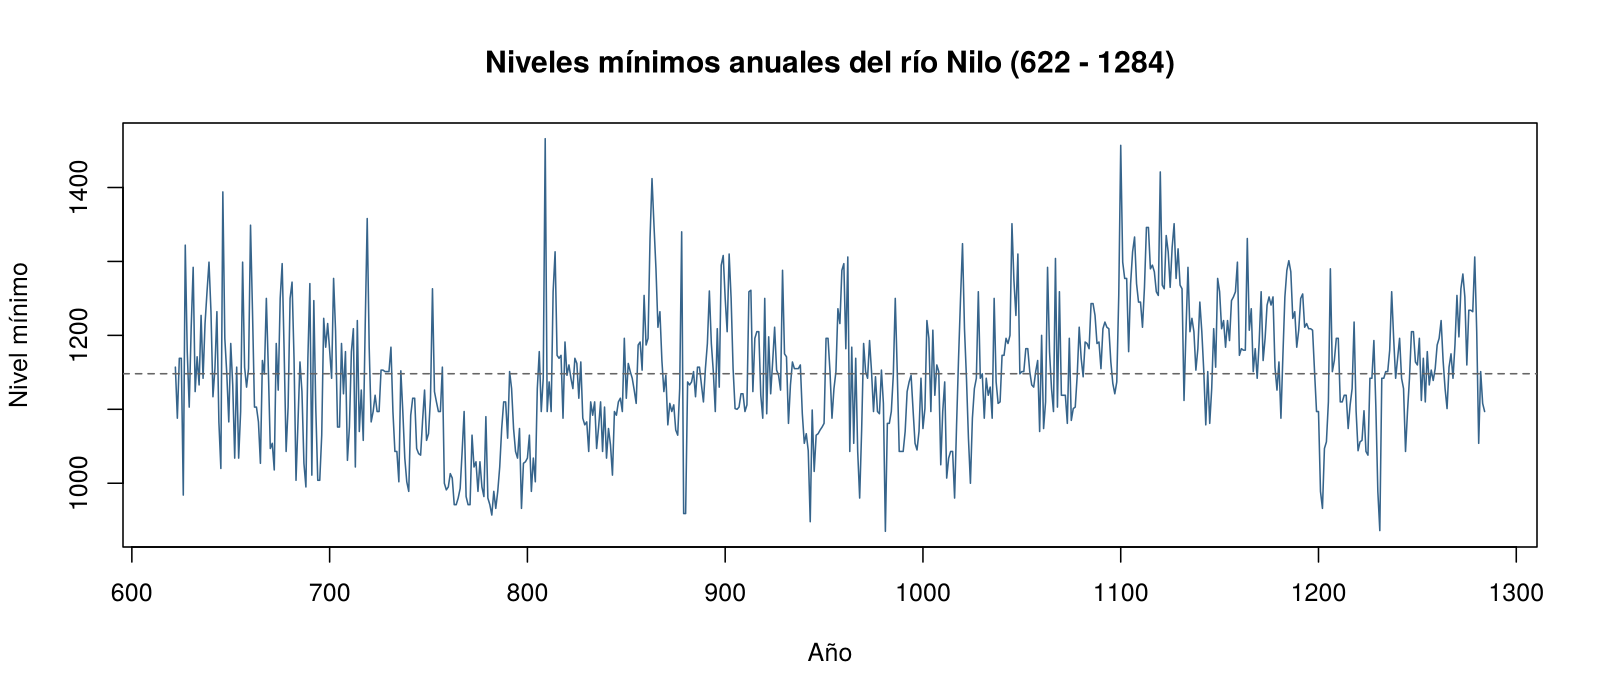
\includegraphics[width=\linewidth]{figuras/serie_nilo.png}
\caption{Niveles m\'inimos anuales del r\'io Nilo, 622 a 1284. La l\'inea punteada es la media de la serie.}
\label{fig:serie}
\end{figure}

\medskip
\noindent\textbf{8.2 Exploraci\'on: ACF y PACF muestrales}

La Figura~\ref{fig:acf} muestra la ACF y la PACF muestrales hasta el rezago 100. La ACF es la se\~nal m\'as clara de memoria larga que tiene la serie. Su primer valor es $\hat\rho(1) = 0.575$, que no es muy grande (en una serie con ra\'iz unitaria estar\'ia muy cerca de 1), pero despu\'es baja much\'isimo m\'as despacio de lo que bajar\'ia en un ARMA: en el rezago 10 todav\'ia vale 0.278, en el rezago 20 vale 0.232 y en el rezago 50 vale 0.135. Las autocorrelaciones siguen por fuera de la banda de significancia ($\pm 1.96/\sqrt{n} = \pm 0.076$) hasta cerca del rezago 75, es decir, la serie parece ``recordar'' lo que pas\'o hace m\'as de 70 a\~nos. La PACF, en cambio, tiene unos pocos valores significativos en los primeros rezagos y despu\'es se queda dentro de la banda.

\begin{figure}[H]
\centering
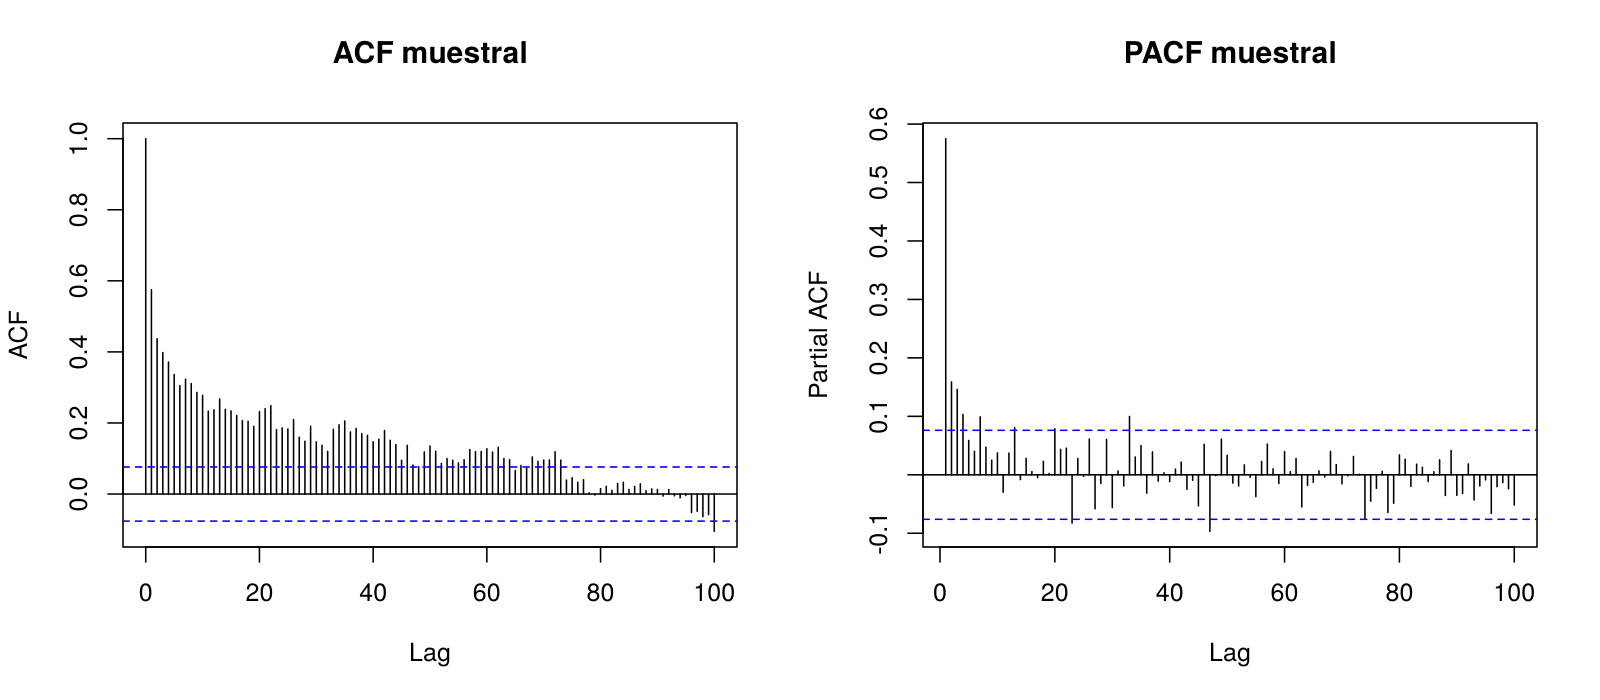
\includegraphics[width=\linewidth]{figuras/acf_pacf_nilo.png}
\caption{ACF y PACF muestrales de la serie del Nilo hasta el rezago 100.}
\label{fig:acf}
\end{figure}

\medskip
\noindent\textbf{8.3 Pruebas de estacionariedad}

La Tabla~\ref{tab:pruebas} resume las pruebas ADF y KPSS. Las dos rechazan su hip\'otesis nula con un p-valor menor a 0.01, lo que a primera vista parece una contradicci\'on: la ADF dice que la serie \emph{no} tiene ra\'iz unitaria y la KPSS dice que la serie \emph{no} es estacionaria. En realidad no hay contradicci\'on, sino que ninguno de los dos modelos que comparan estas pruebas describe bien la serie. La serie es demasiado persistente para ser un ARMA de memoria corta, y no lo suficiente para tener una ra\'iz unitaria. Este resultado es un indicio cl\'asico de memoria larga y es la primera justificaci\'on para usar un ARFIMA.

\begin{table}[H]
\centering
\begin{tabular}{lccl}
\hline
\textbf{Prueba} & \textbf{Estad\'istico} & \textbf{p-valor} & \textbf{Conclusi\'on} \\
\hline
ADF ($H_0$: ra\'iz unitaria) & $-5.03$ & $< 0.01$ & Se rechaza: no hay ra\'iz unitaria \\
KPSS ($H_0$: estacionariedad) & $1.72$ & $< 0.01$ & Se rechaza: no es estacionaria \\
\hline
\end{tabular}
\caption{Pruebas de estacionariedad para la serie del Nilo.}
\label{tab:pruebas}
\end{table}

\medskip
\noindent\textbf{8.4 Estimaci\'on del par\'ametro de memoria $d$}

\emph{Estimador GPH.} La Tabla~\ref{tab:gph} muestra el estimador de Geweke y Porter-Hudak (1983) con tres anchos de banda $m = n^{\alpha}$. Con la propuesta original de los autores, $\alpha = 0.5$, se usan solo $m = 25$ frecuencias y se obtiene $\hat d = 0.504$. Al usar m\'as frecuencias, el estimador cambia bastante y llega a 0.396 con $m = 94$. Esto confirma lo que dijimos en la secci\'on 5.6: el GPH es muy sensible a la elecci\'on de $m$ y tiene errores est\'andar grandes. Aun as\'i, en los tres casos el valor estimado est\'a lejos de cero, lo que apoya la presencia de memoria larga.

\begin{table}[H]
\centering
\begin{tabular}{cccc}
\hline
$\alpha$ & $m = n^{\alpha}$ & $\hat d_{GPH}$ & Error est\'andar asint\'otico \\
\hline
0.5 & 25 & 0.504 & 0.157 \\
0.6 & 49 & 0.537 & 0.105 \\
0.7 & 94 & 0.396 & 0.072 \\
\hline
\end{tabular}
\caption{Estimador GPH de $d$ para distintos anchos de banda.}
\label{tab:gph}
\end{table}

\emph{M\'axima verosimilitud.} Ajustamos los nueve modelos ARFIMA$(p,d,q)$ con $p,q \in \{0,1,2\}$ usando el paquete \texttt{fracdiff}. La Tabla~\ref{tab:arfima} muestra los mejores seg\'un el BIC. En todos los modelos el valor estimado de $d$ est\'a entre 0.35 y 0.39, as\'i que la estimaci\'on de la memoria es bastante estable sin importar la parte ARMA que se agregue. El modelo con menor BIC es el ARFIMA$(0,d,0)$, es decir, el ruido fraccional, que tiene \emph{un solo par\'ametro}. El ARFIMA$(2,d,2)$ tiene el menor AIC, pero al revisar sus coeficientes encontramos que las ra\'ices del polinomio AR y las del polinomio MA pr\'acticamente coinciden, as\'i que las dos partes se cancelan entre s\'i y el modelo est\'a sobreajustado. Por eso escogemos el ARFIMA$(0,d,0)$.

\begin{table}[H]
\centering
\begin{tabular}{lcccc}
\hline
\textbf{Modelo} & $\hat d$ & \textbf{log-verosimilitud} & \textbf{AIC} & \textbf{BIC} \\
\hline
ARFIMA$(0,d,0)$ & 0.393 & $-3757.76$ & 7519.52 & \textbf{7528.52} \\
ARFIMA$(0,d,1)$ & 0.353 & $-3758.06$ & 7522.13 & 7535.62 \\
ARFIMA$(1,d,0)$ & 0.355 & $-3758.16$ & 7522.31 & 7535.80 \\
ARFIMA$(2,d,2)$ & 0.384 & $-3751.00$ & \textbf{7514.00} & 7540.98 \\
\hline
\end{tabular}
\caption{Mejores modelos ARFIMA$(p,d,q)$ estimados por m\'axima verosimilitud, ordenados por BIC.}
\label{tab:arfima}
\end{table}

Para el modelo escogido obtenemos $\hat d = 0.393$, con un error est\'andar asint\'otico de $\sqrt{6/(\pi^2 n)} = 0.030$ y un intervalo de confianza del 95\,\% de $[0.334,\ 0.453]$. El intervalo queda completamente dentro de $(0, 0.5)$, as\'i que, de acuerdo con la Tabla~\ref{tab:d}, la serie del Nilo es \emph{estacionaria con memoria larga}: no necesita diferenciarse, pero tampoco es un ARMA. El exponente de Hurst correspondiente es $\hat H = \hat d + 0.5 = 0.89$, que est\'a bastante por encima del valor de 0.5 que corresponder\'ia a una serie sin memoria larga.

\medskip
\noindent\textbf{8.5 Comparaci\'on con los modelos ARMA y ARIMA}

Sobre la misma serie escogimos el mejor ARMA$(p,q)$ y el mejor ARIMA$(p,1,q)$ con la funci\'on \texttt{auto.arima}. Los resultados est\'an en la Tabla~\ref{tab:comparacion}.

\begin{table}[H]
\centering
\begin{tabular}{lcccc}
\hline
\textbf{Modelo} & \textbf{Par\'ametros} & \textbf{log-verosimilitud} & \textbf{AIC} & \textbf{BIC} \\
\hline
ARFIMA$(0,d,0)$ & 1 & $-3757.76$ & 7519.52 & 7528.52 \\
ARMA$(2,1)$ & 3 & $-3756.37$ & 7522.74 & 7545.23 \\
ARIMA$(1,1,3)$ & 4 & $-3752.93$ & 7515.86* & 7538.33* \\
\hline
\multicolumn{5}{l}{\footnotesize * Calculados sobre la serie diferenciada, no comparables con los otros dos modelos.}
\end{tabular}
\caption{Modelos ARFIMA, ARMA y ARIMA ajustados a la serie del Nilo. Los par\'ametros no incluyen la media ni la varianza.}
\label{tab:comparacion}
\end{table}
Vale la pena anotar que estos dos modelos son exactamente los que propone \texttt{auto.arima} cuando lo dejamos escoger tambi\'en el orden de diferenciaci\'on. Esta funci\'on decide $d$ con una prueba de ra\'iz unitaria: con la prueba KPSS, que es la que usa por defecto, escoge $d = 1$ y llega al ARIMA$(1,1,3)$; con la prueba ADF escoge $d = 0$ y llega al ARMA$(2,1)$. Es decir, el modelo autom\'atico cambia por completo seg\'un la prueba que se use, porque solo puede escoger entre no diferenciar y diferenciar una vez. Esto muestra bien el problema que resuelve el ARFIMA: con una serie de memoria larga, la decisi\'on entre $d = 0$ y $d = 1$ no tiene una respuesta correcta, y lo razonable es estimar un $d$ intermedio.

Lo primero que llama la atenci\'on es la parsimonia. Para describir la serie, el ARMA necesita tres par\'ametros ($\phi_1 = 1.28$, $\phi_2 = -0.30$ y $\theta_1 = -0.85$), y aun as\'i tiene un AIC y un BIC peores que los del ARFIMA$(0,d,0)$, que usa uno solo. Adem\'as, el ARMA tiene una ra\'iz autorregresiva muy cerca del c\'irculo unitario, que es la forma en que un modelo de memoria corta intenta imitar una persistencia que en realidad es de largo plazo. El ARIMA, por su lado, no se puede comparar con los criterios de informaci\'on, porque su verosimilitud se calcula sobre la serie diferenciada y no sobre la original. Por eso la comparaci\'on justa entre los tres es la de pron\'ostico (secci\'on 8.7).

La Figura~\ref{fig:espectro} compara los modelos en el dominio de las frecuencias, que es donde la diferencia entre memoria corta y larga se ve m\'as clara. En escala logar\'itmica en ambos ejes, la densidad espectral del ARFIMA$(0,d,0)$ es pr\'acticamente una recta con pendiente $-2\hat d$, que sigue creciendo a medida que la frecuencia se acerca a cero, tal como dice la ecuaci\'on~(3). El espectro del ARMA, en cambio, es acotado y tiene que aplanarse cerca del origen. En el rango de frecuencias que tiene la muestra los dos modelos se parecen bastante, pero la forma en la que lo logran es muy distinta: el ARFIMA lo hace con un solo par\'ametro que describe directamente la memoria, y el ARMA lo hace combinando tres par\'ametros para aproximar esa misma forma.

\begin{figure}[H]
\centering
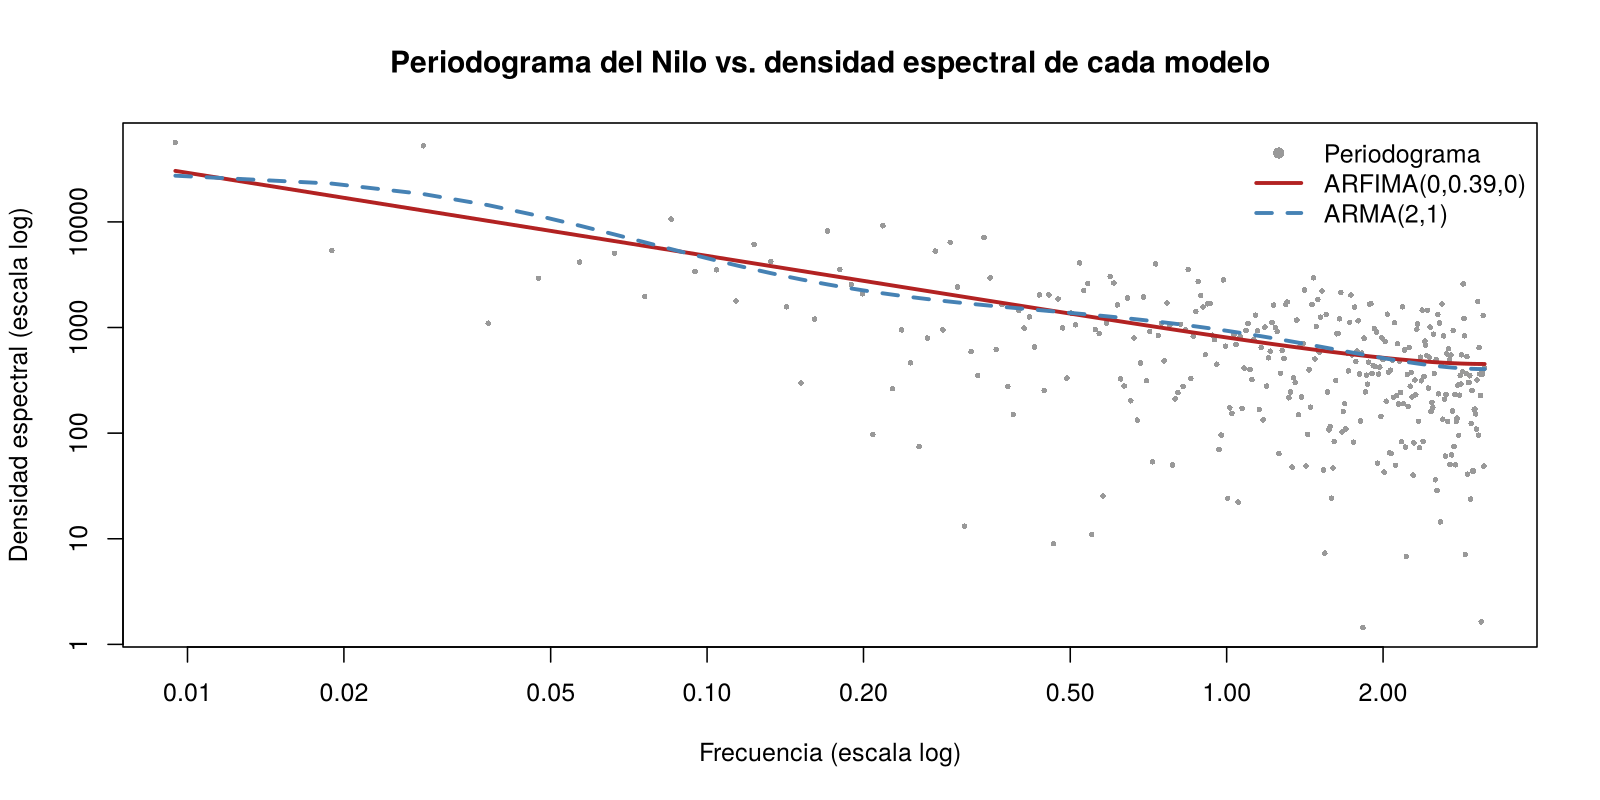
\includegraphics[width=\linewidth]{figuras/espectro_modelos.png}
\caption{Periodograma de la serie del Nilo (puntos) y densidad espectral estimada de los modelos ARFIMA$(0,d,0)$ y ARMA$(2,1)$, en escala log-log.}
\label{fig:espectro}
\end{figure}

\medskip
\noindent\textbf{8.6 Diagn\'ostico de los residuales}

Para cada modelo aplicamos la prueba de Ljung-Box con 20 rezagos, cuya hip\'otesis nula es que los residuales son ruido blanco. Los p-valores fueron 0.866 para el ARFIMA$(0,d,0)$, 0.838 para el ARMA$(2,1)$ y 0.834 para el ARIMA$(1,1,3)$, as\'i que en ning\'un caso se rechaza la hip\'otesis nula. La Figura~\ref{fig:residuales} muestra los residuales del ARFIMA y su ACF, que se queda dentro de las bandas de significancia. Es decir, con un solo par\'ametro el ARFIMA logra capturar toda la dependencia de la serie, algo que el ARMA y el ARIMA consiguen solo con tres y cuatro par\'ametros.

\begin{figure}[H]
\centering
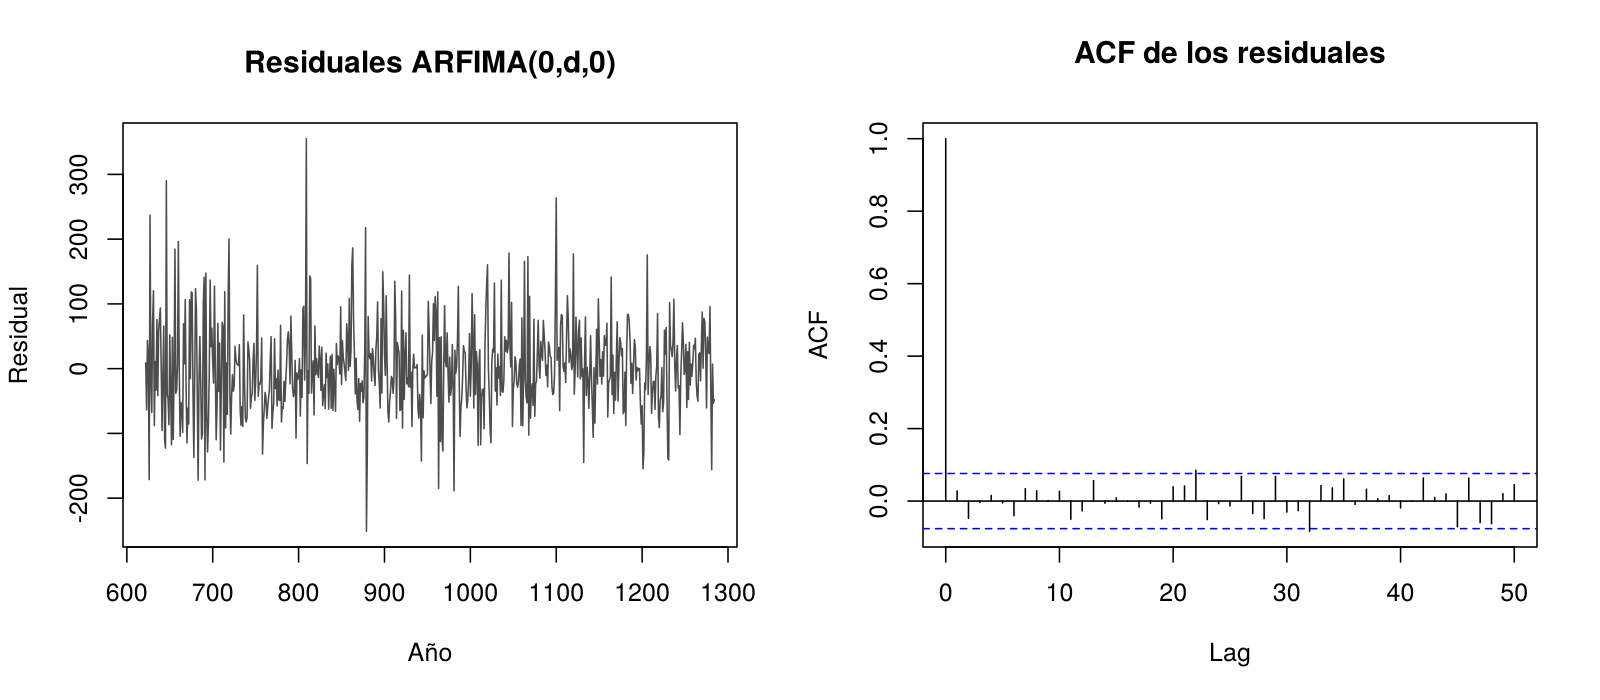
\includegraphics[width=\linewidth]{figuras/residuales_arfima.png}
\caption{Residuales del modelo ARFIMA$(0,d,0)$ y su ACF muestral.}
\label{fig:residuales}
\end{figure}

\medskip
\noindent\textbf{8.7 Pron\'ostico fuera de muestra}

Para comparar los tres modelos en igualdad de condiciones, separamos las \'ultimas 50 observaciones (a\~nos 1235 a 1284) como conjunto de prueba y estimamos los modelos solo con las 613 observaciones anteriores. Como referencia usamos el pron\'ostico m\'as sencillo posible: predecir todos los a\~nos con la media del entrenamiento. Los errores est\'an en la Tabla~\ref{tab:pronostico}.

\begin{table}[H]
\centering
\begin{tabular}{lcccc}
\hline
 & \multicolumn{2}{c}{\textbf{A un paso}} & \multicolumn{2}{c}{\textbf{A varios pasos (50 a\~nos)}} \\
\textbf{Modelo} & RMSE & MAE & RMSE & MAE \\
\hline
ARFIMA$(0,d,0)$ & \textbf{50.10} & \textbf{39.85} & 62.59 & 49.30 \\
ARMA$(2,1)$ & 50.79 & 40.71 & 68.90 & 55.99 \\
ARIMA$(1,1,3)$ & 50.71 & 40.54 & 74.77 & 60.77 \\
Media del entrenamiento & 60.73 & 46.94 & \textbf{60.73} & \textbf{46.94} \\
\hline
\end{tabular}
\caption{Errores de pron\'ostico sobre las \'ultimas 50 observaciones de la serie.}
\label{tab:pronostico}
\end{table}

\emph{Pron\'ostico a un paso.} Aqu\'i cada a\~no se pronostica con toda la informaci\'on disponible hasta el a\~no anterior. Los tres modelos le ganan claramente a la media, con una reducci\'on del RMSE de alrededor del 17\,\%, lo que muestra que la dependencia de la serie s\'i sirve para predecir. El ARFIMA tiene el menor error de los tres, aunque la diferencia con el ARMA y el ARIMA es peque\~na.

\emph{Pron\'ostico a varios pasos.} Aqu\'i se pronostican los 50 a\~nos de una vez, desde el final del entrenamiento. La Figura~\ref{fig:pronostico} muestra que las diferencias entre los modelos son m\'as grandes. El ARIMA, que supone que los choques son permanentes, deja el pron\'ostico casi plano en un nivel bajo y es el que m\'as se equivoca. El ARMA y el ARFIMA s\'i regresan hacia la media, pero el ARFIMA lo hace de forma m\'as gradual, como corresponde a un proceso con memoria larga, y tiene un error claramente menor que el del ARMA. Sin embargo, a un horizonte tan largo ninguno de los tres modelos le gana a la media sola, que tiene el menor RMSE. Esto tiene sentido: cuando se pronostica muy lejos, cualquier modelo estacionario termina convergiendo a la media, as\'i que la ventaja de modelar la dependencia se va perdiendo con el horizonte. Lo importante es que, de los tres modelos, el ARFIMA es el que menos se aleja de ese comportamiento.

\begin{figure}[H]
\centering
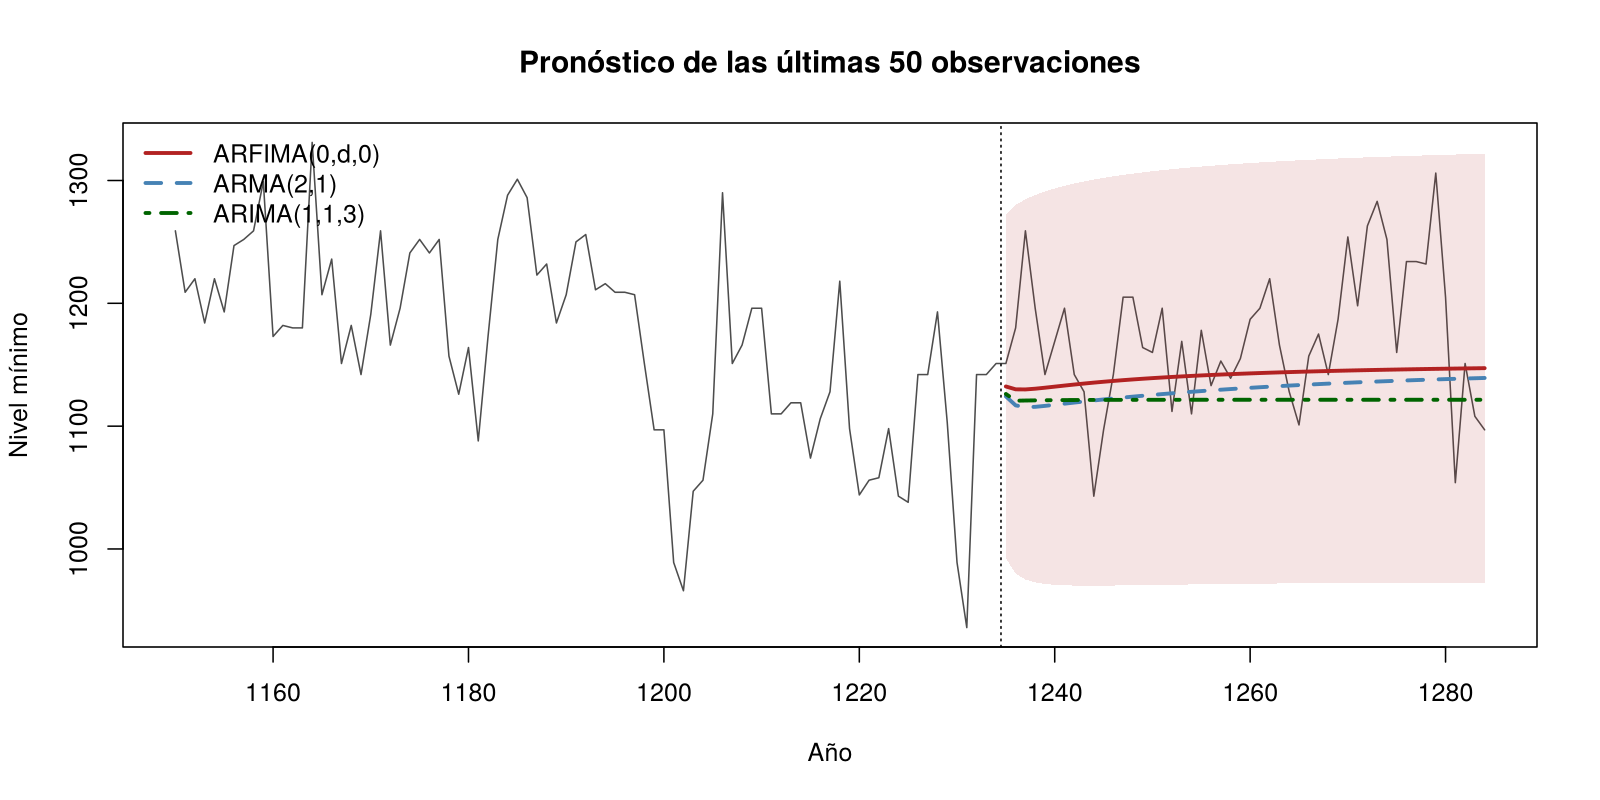
\includegraphics[width=\linewidth]{figuras/pronosticos.png}
\caption{Pron\'ostico a varios pasos de las \'ultimas 50 observaciones con los tres modelos. La franja sombreada es el intervalo de predicci\'on del 95\,\% del ARFIMA$(0,d,0)$.}
\label{fig:pronostico}
\end{figure}
\medskip
\item \textbf{CONCLUSIONES}

\medskip
\noindent\textbf{Lo que dec\'ia la teor\'ia y lo que encontramos}

Todas las se\~nales de memoria larga que describimos en el marco te\'orico aparecieron en la serie del Nilo. La ACF muestral baj\'o de forma lenta y se mantuvo significativa hasta cerca del rezago 75, en lugar de caer r\'apido como en un ARMA. El periodograma creci\'o cerca de la frecuencia cero siguiendo casi una recta en escala log-log, que es justo la forma que predice la ecuaci\'on (3). Y las pruebas ADF y KPSS rechazaron al mismo tiempo, lo que muestra que la serie no encaja ni en el mundo de la memoria corta ni en el de la ra\'iz unitaria, que son las dos \'unicas opciones que ofrecen los modelos vistos en el curso.

El par\'ametro de memoria estimado, $\hat d = 0.393$, qued\'o dentro del intervalo $(0, 0.5)$ con todo y su intervalo de confianza. Seg\'un la Tabla~\ref{tab:d}, eso significa que el Nilo es una serie estacionaria con memoria larga: no hace falta diferenciarla, pero tampoco se puede tratar como un ARMA. El exponente de Hurst correspondiente, $\hat H = 0.89$, confirma con un modelo estad\'istico moderno el mismo efecto que Hurst describi\'o hace m\'as de setenta a\~nos estudiando este r\'io.

Tambi\'en se cumpli\'o lo que dijimos sobre los m\'etodos de estimaci\'on. El estimador GPH dio valores entre 0.40 y 0.54 seg\'un cu\'antas frecuencias se usaran, as\'i que es \'util para detectar la memoria larga pero poco preciso para cuantificarla. La m\'axima verosimilitud, en cambio, dio valores de $d$ muy parecidos (entre 0.35 y 0.39) sin importar la parte ARMA que se agregara al modelo.

Frente a los modelos del curso, el ARFIMA$(0,d,0)$ describi\'o la serie con un solo par\'ametro, mientras que el ARMA necesit\'o tres y el ARIMA cuatro para dejar residuales que tambi\'en pasaran la prueba de Ljung-Box. En el pron\'ostico, el ARFIMA tuvo el menor error de los tres modelos tanto a un paso como a varios pasos, aunque a un paso la ventaja fue peque\~na y a 50 a\~nos ninguno de los modelos le gan\'o a la media de la serie. Este \'ultimo resultado nos parece importante: la memoria larga mejora el pron\'ostico frente a ARMA y ARIMA, pero no hace milagros a horizontes muy largos, donde cualquier modelo estacionario termina convergiendo a la media.

\medskip
\noindent\textbf{Ventajas de los modelos ARFIMA}
\begin{itemize}
\item Llenan el vac\'io entre los ARMA ($d = 0$) y los ARIMA ($d = 1$). En lugar de escoger entre no diferenciar o diferenciar una vez, el modelo estima cu\'anto hay que diferenciar, y as\'i evita la sobrediferenciaci\'on.
\item Son parsimoniosos. Un solo par\'ametro, $d$, describe toda la dependencia de largo plazo, que un ARMA solo puede imitar con varios par\'ametros y con ra\'ices muy cerca del c\'irculo unitario.
\item Separan los dos tipos de dependencia: $d$ se encarga del largo plazo y la parte ARMA del corto plazo, y cada uno se puede interpretar por aparte.
\item El par\'ametro $d$ tiene una interpretaci\'on directa, tanto por sus rangos (Tabla~\ref{tab:d}) como por su relaci\'on con el exponente de Hurst.
\item Sus pron\'osticos regresan a la media de forma gradual, lo que en nuestra aplicaci\'on se tradujo en menores errores que los de ARMA y ARIMA.
\end{itemize}

\medskip
\noindent\textbf{Desventajas de los modelos ARFIMA}
\begin{itemize}
\item Son m\'as dif\'iciles de estimar. La verosimilitud exacta es costosa de calcular y en la pr\'actica se usan aproximaciones. Adem\'as, encontramos que el error est\'andar de $d$ que reporta el paquete \texttt{fracdiff} es poco confiable, y tuvimos que usar el error asint\'otico te\'orico.
\item Los estimadores semiparam\'etricos, como el GPH, dependen mucho de decisiones arbitrarias como el n\'umero de frecuencias $m$.
\item Necesitan series largas. Para distinguir la memoria larga de una memoria corta muy persistente hacen falta muchas observaciones; la serie del Nilo tiene 663, y no todas las series con las que se trabaja en la pr\'actica son tan largas.
\item Un cambio estructural en la media de una serie puede producir una ACF que decae lento y hacer que parezca tener memoria larga cuando en realidad no la tiene.
\item Son menos conocidos y no vienen en herramientas de uso diario como \texttt{auto.arima}, as\'i que requieren paquetes adicionales y m\'as cuidado por parte del analista.
\end{itemize}

\medskip
\noindent\textbf{Comentario final}

Los modelos ARFIMA no reemplazan a los ARMA y ARIMA, sino que los complementan. Cuando una serie muestra autocorrelaciones peque\~nas pero muy persistentes, o cuando las pruebas de ra\'iz unitaria y de estacionariedad se contradicen, vale la pena considerar un ARFIMA antes de forzar la serie en uno de los dos extremos que vimos en el curso. En el caso del Nilo, el modelo no solo ajust\'o mejor con menos par\'ametros, sino que permiti\'o medir con un n\'umero el fen\'omeno que dio origen a toda esta teor\'ia.
\medskip
\item \textbf{REFERENCIAS BIBLIOGR{\'A}FICAS}

\begin{list}{}{\setlength{\leftmargin}{1.5em}\setlength{\itemindent}{-1.5em}\setlength{\itemsep}{0.4em}}

\item Geweke, J. y Porter-Hudak, S. (1983). The estimation and application of long memory time series models. \emph{Journal of Time Series Analysis}, 4(4), 221--238. \url{https://doi.org/10.1111/j.1467-9892.1983.tb00371.x}

\item Granger, C. W. J. y Joyeux, R. (1980). An introduction to long-memory time series models and fractional differencing. \emph{Journal of Time Series Analysis}, 1(1), 15--29. \url{https://doi.org/10.1111/j.1467-9892.1980.tb00297.x}

\item Haslett, J. y Raftery, A. E. (1989). Space-time modelling with long-memory dependence: Assessing Ireland's wind power resource. \emph{Applied Statistics}, 38(1), 1--50. \url{https://doi.org/10.2307/2347679}

 \item Hosking, J. R. M. (1981). Fractional differencing. \emph{Biometrika}, 68(1), 165--176.
 \url{https://doi.org/10.1093/biomet/68.1.165}

\item Hurst, H. E. (1951). Long-term storage capacity of reservoirs. \emph{Transactions of the American Society of Civil Engineers}, 116, 770--808.

\item Maechler, M., Fraley, C., Hyndman, R., Leisch, F., Lemonte, A. y Reisen, V. (2026). \emph{fracdiff: Fractionally Differenced ARIMA aka ARFIMA(P,d,q) Models} (versi\'on 1.5-4) [Paquete de R]. \url{https://doi.org/10.32614/CRAN.package.fracdiff}

\item Shumway, R. H. y Stoffer, D. S. (2017). \emph{Time Series Analysis and Its Applications: With R Examples} (4a ed.). Springer.

\item Toussoun, O. (1925). M\'emoire sur l'histoire du Nil. \emph{M\'emoires de l'Institut d'\'Egypte}, 18, 366--404.

\end{list}
\medskip
\end{enumerate}
\end{document}
